\section{Introducci\'on}
Toda se\~nal enviada por un sistema de comunicaci\'on sufre perturbaciones durante el proceso de transmisi\'on, y es por eso que se desea reducir el error de la informaci\'on recibida.
Un modelo discreto sencillo de un sistema de comunicaciones es el siguiente. Peri\'odicamente, cada T segundos el transmisor env\'ia un dato $s_k$ considerando como instante inicial a $t = 0$. Luego, la informaci\'on es modificada por el canal a través de su "respuesta impulsiva". Esto es la respuesta del sistema (en este caso, el canal) frente a una se\~nal de entrada en particular que se conoce como impulso unitario \'o delta de dirac. Matem\'aticamente, esto permite expresar la salida de un sistema en general como la convoluci\'on de su respuesta impulsiva con la se\~nal de entrada.
A su vez, la señal transmitida es afectada por ruido blanco Gaussiano aditivo , donde $N_k \sim cN(0,\sigma)$. Entonces, peri\'odicamente la informaci\'on recibida es 

\begin{equation*} 
r_n = \sum_{k=0}^{L-1} h_k s_{n-k} + N_n 
\end{equation*} 

Donde $h$  es la respuesta impulsiva previamente mencionada. Matricialmente, esto se puede expresar de dos formas distintas:

\begin{equation}  
\vec{r} = H \vec{s} + \vec{N} 
\label{eq: r=hs+n}
\end{equation} 

\begin{equation} 
\vec{r} = S \vec{h} + \vec{N} 
\label{eq: r=sh+n}
\end{equation} 

Siendo en todos los casos 
\begin{itemize}
	\item \textbf{h} referente a información del canal
	\item \textbf{s} referente a información de la señal original
	\item \textbf{n} referente al ruido agregado a la señal
	\item \textbf{r} referente a la señal recibida
\end{itemize}
	
%-------------------------------------------------------------------------------------------------------------------------
\section{Estimaci\'on de la se\~nal enviada}

Es necesario hacer una estimaci\'on de dos cosas distintas. Por un lado se debe estimar el canal ($\vec{h}$) y por otro lado, la imagen original  ($\vec{s}$).

%----------------------------------------------
\subsection{Estimaci\'on del canal de comunicaci\'on}

Primero se hace una estimaci\'on de $\vec{h}$ con el m\'etodo de cuadrados m\'inimos, empleando la descomposici\'on de Cholesky, como se explica a continuaci\'on.  Para averiguar $\vec{h}$ a partir de la ecuaci\'on (\ref{eq: r=sh+n}), se considera que la media del ruido $N$ es cero, y as\'i se obtiene una nueva ecuaci\'on a partir de la cu\'al se proceder\'a:

\begin{equation} 
\vec{r} = S \vec{h}
\label{eq: r=sh} 
\end{equation} 

Para utilizar el m\'etodo de Cholesky en una ecuaci\'on del tipo $\vec{b} = A \vec{h}$ es necesario que la matriz $A$ sea cuadrada, sim\'etrica y definida positiva. Pero en nuestro caso,  en su lugar tenemos a la matriz $S$ que no es  cuadrada. Como necesitamos una matriz que cumpla estas condiciones, multiplicamos ambos lados de la ecuaci\'on (\ref{eq: r=sh}) por $S^T$:

\begin{equation} 
S^T \vec{r} = S^T S \vec{h} 
\end{equation} 

Llamamos  $S^T \vec{r} = \vec{b}$ y  $S^T S = A$, y obtenemos la expresi\'on:

\begin{equation} 
\vec{b} = A \vec{h} 
\label{eq: b=Ah} 
\end{equation} 

En esta nueva ecuaci\'on (\ref{eq: b=Ah}), la matriz A cumple con las caracter\'isticas para implementar el m\'etodo de Cholesky, el cual consiste en encontrar las matrices $L$ y $L^T$ triangulares, tales que $A = L L^T$, para simplificar la resoluci\'on de la ecuaci\'on. Una vez averiguadas las matrices  $L$ y $L^T$,en la ecuaci\'on (\ref{eq: b=Ah}) reemplazamos la matriz $A$ por el producto entre ellas y obtenemos:

\begin{equation} 
\vec{b} = L L^T \vec{h} 
\label{eq: b=LLth}
\end{equation} 

Llamamos $\vec{y} = L^T \vec{h}$ y lo reemplazamos en la ecuaci\'on (\ref{eq: b=LLth}), de modo que:

\begin{equation} 
\vec{b} = L \vec{y}
\label{eq: b=Ly}
\end{equation} 

A partir de la ecuaci\'on (\ref{eq: b=Ly}) obtenemos $ \vec{y}$ realizando sustituci\'on Forward. Finalmente, dado que, como se mencion\'o previamente:

 \begin{equation} 
\vec{y} = L^T \vec{h} 
\label{eq: y=Lth}
\end{equation}

se despeja $\vec{h}$ de la ecuaci\'on (\ref{eq: y=Lth}) haciendo una sustituci\'on Backward. La ventaja de implementar el m\'etodo de Cholesky para la ecuaci\'on resuelta es que se terminan resolviendo dos ecuaciones en las que la matriz involucrada (ya sea $L$ o $L^T$) es una matriz triangular.

%----------------------------------------------
\subsection{Estimaci\'on de la imagen original}

La estimaci\'on de la imagen original $\vec{s}$, se hace a partir de la ecuaci\'on (\ref{eq: r=hs+n}), de una manera distinta a la implementada para la estimaci\'on de  $\vec{h}$. A pesar de que tambi\'en se realiza haciendo cuadrados m\'inimos, asumimos que el nivel de ruido es conocido y usamos otro m\'etodo  conocido como Linear Minimum Square Error (LMMSE). Si bien no es lo correcto, asumimos que las m\'inimas unidades transmitidas en la se\~nal enviada son independientes entre s\'i, simplemente para que la resoluci\'on sea m\'as sencilla. 


%EN ALGUNA PARTE HAY QUE MENCIONAR QUE SE HACE UNA SECUENCIA DE ENTRENAMIENTO!!!!!!!!!!!!!!!!!!!!!%
%%%
Para ver como funciona todo lo explicado hasta aqu\'i, se env\'ia la imagen de Lena con un ruido de un desv\'io est\'andar de 1. A continuaci\'on se observan los resultados de la transmisi\'on de la imagen de Lena en escala de grises.
 

\begin{figure}[H]
	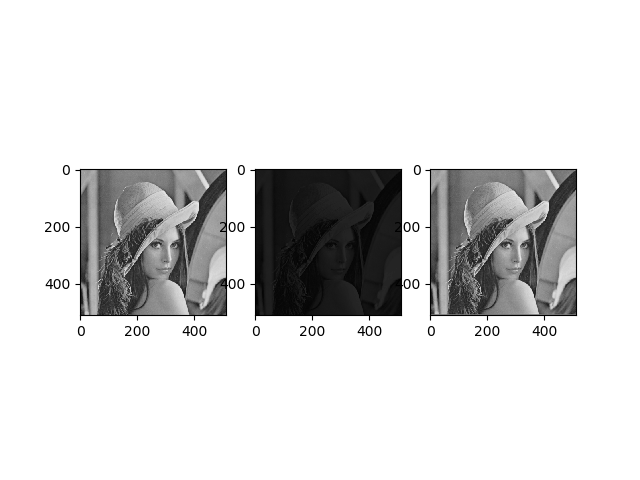
\includegraphics[scale=1]{Imagenes/E32S01}
	\centering
\end{figure}
 
\begin{figure}[H]
	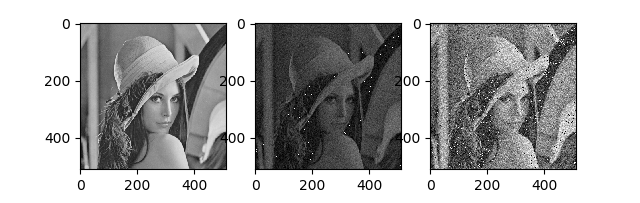
\includegraphics[scale=1]{Imagenes/E32S10}
	\centering
\end{figure}

\begin{figure}[H]
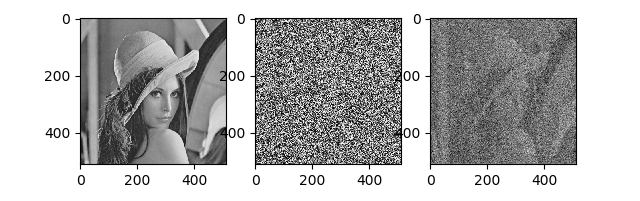
\includegraphics[scale=1]{Imagenes/E32S100}
\centering
\end{figure}

\begin{figure}[H]
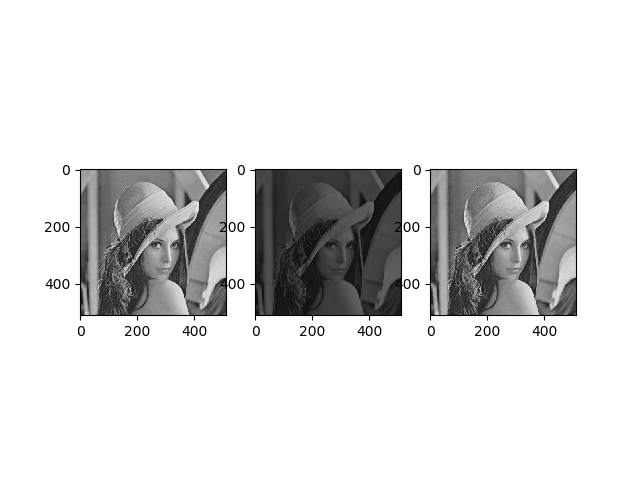
\includegraphics[scale=1]{Imagenes/E1024S01}
\centering
\end{figure}

\begin{figure}[H]
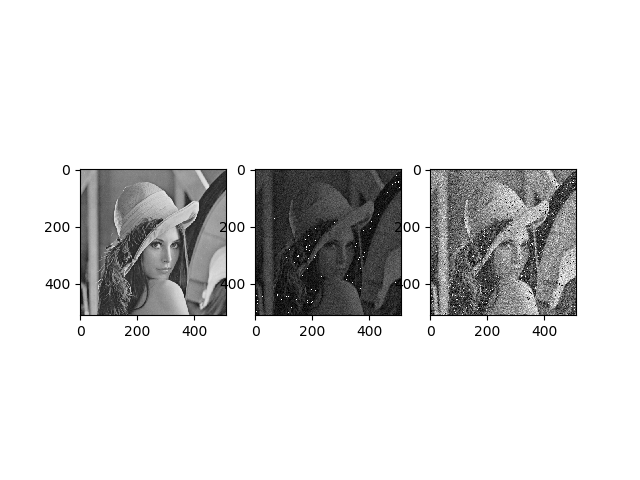
\includegraphics[scale=1]{Imagenes/E1024S10}
\centering
\end{figure}

\begin{figure}[H]
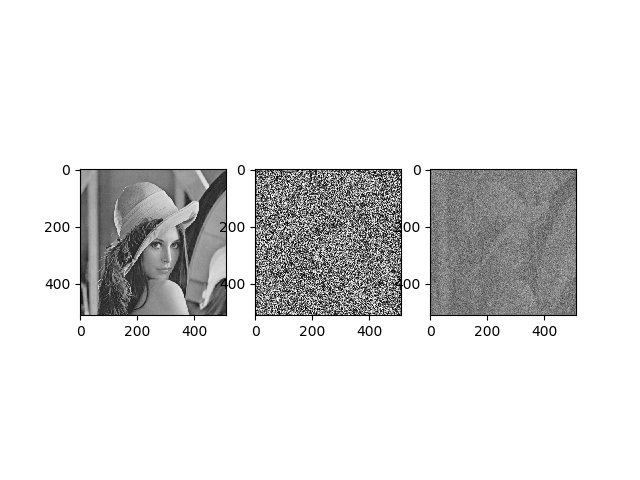
\includegraphics[scale=1]{Imagenes/E1024S100}
\centering
\end{figure}

%explicar los resultados haciendo comparaciones entre los resultados y la imagen real, y entre los resultados y el ruido y entre los resultados distintos debiedo a la variable que se fue cambiando.

En base a los resultados obtenidos, se puede establecer una relaci\'on 
entre la dispersi\'on del ruido y la imagen recuperada respecto de la original. Para una misma longitud de entrenamiento, si el ruido presente en el canal posee mayor dispersi\'on, quiere decir que puede tomar una distribuci\'on de valores m\'as amplia. Por ello, resulta m\'as dificultoso recuperar la informaci\'on original de la imagen si aletar, y a la salida se la ve afectada por el ruido en mayor medida en cuanto $\sigma$ aumenta.

